%% ============================================================
%%  Relatório de Pós-Graduação — Análise de Séries Temporais
%%  Tema: Consumo de Eletricidade na Alemanha (ENTSO-E)
%%
%%  COMO COMPILAR:
%%    xelatex Relatorio_Electricity_Germany.tex
%%    biber   Relatorio_Electricity_Germany
%%    xelatex Relatorio_Electricity_Germany.tex
%%    xelatex Relatorio_Electricity_Germany.tex
%%
%%  Figuras geradas pelo script analysis.py (mesma pasta):
%%    fig_serie.png
%%    fig_stl.png
%%    fig_fac_facp.png
%%    fig_fac_facp_diff.png
%%    fig_criterios.png
%%    fig_diagnostico.png
%%    fig_previsao.png
%% ============================================================
\documentclass[12pt, a4paper]{article}

% ── Fontes e codificação (XeLaTeX — UTF-8 nativo) ────────────
\usepackage{fontspec}
\setmainfont{Latin Modern Roman}
\usepackage{microtype}

% ── Referências ──────────────────────────────────────────────
\usepackage[backend=biber, style=numeric, sorting=nty, sortcites=true]{biblatex}
\addbibresource{Reference_Electricity.bib}

% ── Layout ───────────────────────────────────────────────────
\usepackage[top=2.5cm, bottom=2.5cm, left=3.0cm, right=2.5cm]{geometry}
\usepackage{setspace}
\onehalfspacing
\setlength{\parindent}{1.25cm}
\setlength{\parskip}{0pt}

% ── Matemática ───────────────────────────────────────────────
\usepackage{amsmath, amssymb}

% ── Figuras e tabelas ────────────────────────────────────────
\usepackage{graphicx}
\usepackage{float}
\usepackage{booktabs}
\usepackage{array}
\usepackage{tabularx}
\usepackage[table]{xcolor}
\usepackage{subcaption}

% ── Código Python ────────────────────────────────────────────
\usepackage{listings}
\definecolor{codebg}{RGB}{240,240,240}
\definecolor{codeframe}{RGB}{180,180,180}
\definecolor{codekw}{RGB}{0,0,180}
\definecolor{codecomment}{RGB}{0,120,0}
\definecolor{codestr}{RGB}{160,0,0}
\lstdefinestyle{python}{
  language=Python,
  backgroundcolor=\color{codebg},
  frame=single,
  framerule=0.5pt,
  rulecolor=\color{codeframe},
  basicstyle=\small\ttfamily,
  keywordstyle=\color{codekw}\bfseries,
  commentstyle=\color{codecomment}\itshape,
  stringstyle=\color{codestr},
  breaklines=true,
  showstringspaces=false,
  numbers=none,
  xleftmargin=8pt,
  xrightmargin=8pt,
  aboveskip=6pt,
  belowskip=6pt
}
\lstset{style=python}

% ── Cabeçalhos e rodapés ─────────────────────────────────────
\usepackage{fancyhdr}
\pagestyle{fancy}
\fancyhf{}
\fancyhead[L]{\small\itshape Consumo de Eletricidade na Alemanha}
\fancyhead[R]{\small\itshape Análise de Séries Temporais}
\fancyfoot[C]{\small\thepage}
\renewcommand{\headrulewidth}{0.4pt}

% ── Hiperlinks ───────────────────────────────────────────────
\usepackage[hidelinks]{hyperref}

% ── Cores ────────────────────────────────────────────────────
\definecolor{azulescuro}{RGB}{31,56,100}
\definecolor{azulmedio}{RGB}{44,95,138}
\definecolor{cinzaclaro}{RGB}{235,243,251}
\definecolor{verdeescuro}{RGB}{0,100,0}

% ── Formatação de seções ─────────────────────────────────────
\usepackage{titlesec}
\titleformat{\section}
  {\large\bfseries\color{azulescuro}}
  {\thesection.}{0.6em}{}
  [\vspace{-0.25em}\textcolor{azulmedio}{\rule{\linewidth}{0.7pt}}]
\titleformat{\subsection}
  {\normalsize\bfseries\color{azulmedio}}
  {\thesubsection.}{0.5em}{}
\titlespacing{\section}{0pt}{18pt}{8pt}
\titlespacing{\subsection}{0pt}{12pt}{4pt}

% ── Legendas ─────────────────────────────────────────────────
\usepackage{caption}
\captionsetup{
  font=small,
  labelfont=bf,
  labelsep=period,
  justification=justified
}

% ── Caixa de destaque ────────────────────────────────────────
\usepackage{tcolorbox}
\tcbuselibrary{skins}
\newtcolorbox{caixaDestaque}[1]{
  colback=cinzaclaro,
  colframe=azulmedio,
  fonttitle=\small\bfseries,
  title=#1,
  left=8pt, right=8pt, top=5pt, bottom=5pt,
  boxrule=0.7pt
}

% ── TikZ ─────────────────────────────────────────────────────
\usepackage{tikz}
\usetikzlibrary{shapes.geometric, arrows.meta, positioning}
\tikzstyle{block}      = [rectangle, draw, fill=gray!10,
    text width=8cm, text centered, minimum height=1cm]
\tikzstyle{line}       = [draw, -{Latex}]
\tikzstyle{decision}   = [diamond, draw, fill=gray!10,
    text width=2.5cm, text centered, inner sep=1pt]
\tikzstyle{terminator} = [ellipse, draw, fill=gray!10,
    text width=3cm, text centered, minimum height=1cm]

% ─────────────────────────────────────────────────────────────
\begin{document}

% ══════════════════════════════════════════════════════════════
%  CAPA
% ══════════════════════════════════════════════════════════════
\begin{titlepage}
  \centering
  \vspace*{1cm}

  {\large\scshape\color{azulescuro}
    Universidade Estadual de Campinas \\
    Instituto de Matemática, Estatística e Computação Científica}\\[0.3em]
  {\normalsize\itshape ME607 -- Séries Temporais}\\[0.2em]
  {\small\itshape Semestre 01/2026 -- Trabalho Final}

  \vspace{2.5cm}

  {\LARGE\bfseries\color{azulescuro}
    Modelagem SARIMA do Consumo\\[0.3em]
    de Eletricidade na Alemanha}

  \vspace{1cm}

  {\large\itshape
    Análise Completa de Séries Temporais\\[0.4em]
    com Dados Mensais da ENTSO-E (2006--2023)}

  \vspace{3cm}

  {\normalsize
    [Nome do Aluno] -- RA: [XXXXXX]
  }

  \vfill
  {\normalsize \today}
\end{titlepage}

\thispagestyle{fancy}

% ══════════════════════════════════════════════════════════════
%  RESUMO
% ══════════════════════════════════════════════════════════════
\begin{abstract}
\noindent
Este trabalho apresenta uma análise estatística completa da série mensal de consumo
total de eletricidade na Alemanha, disponibilizada pela \textit{European Network of
Transmission System Operators for Electricity} (ENTSO-E), cobrindo o período de
janeiro de 2006 a dezembro de 2023 (216 observações mensais). A série exibe tendência
decrescente suave, forte sazonalidade anual determinada pelo ciclo de aquecimento e
arrefecimento, e uma intervenção estrutural claramente identificável em 2020 associada
à pandemia de COVID-19. A metodologia de Box-Jenkins \cite{BoxTimeSeries} é seguida
sistematicamente nas etapas de análise exploratória, decomposição sazonal, testes de
estacionaridade, identificação, estimação e diagnóstico de modelos da classe
$\mathrm{SARIMA}(p,d,q)(P,D,Q)_{12}$. Toda a análise é conduzida em Python, utilizando
os pacotes \texttt{statsmodels}, \texttt{pmdarima}, \texttt{pandas},
\texttt{matplotlib} e \texttt{scipy}. Uma discussão crítica das vantagens, limitações
e extensões do modelo encerra o trabalho.
\end{abstract}

\vspace{0.5cm}
\noindent\textbf{Palavras-chave:} Consumo de Eletricidade; Alemanha; SARIMA; Sazonalidade;
Análise de Intervenção; Box-Jenkins.

\vspace{0.5cm}
\tableofcontents
\newpage

% ══════════════════════════════════════════════════════════════
\section{Introdução}
% ══════════════════════════════════════════════════════════════

A previsão e modelagem do consumo de energia elétrica constituem problemas de grande
relevância prática para operadores de redes de transmissão, reguladores e formuladores
de política energética. Séries de consumo elétrico apresentam características que as
tornam particularmente adequadas para a metodologia de Box-Jenkins
\cite{SeriesTemporaisMoretti}: sazonalidade anual bem definida, tendência de médio prazo
relacionada a fatores estruturais como eficiência energética e composição industrial, e
perturbações exógenas identificáveis como recessões econômicas ou pandemias.

A Alemanha representa um caso de especial interesse neste contexto. Sendo a maior
economia da Europa, seu sistema elétrico integra uma crescente parcela de energias
renováveis (eólica e solar), cuja natureza intermitente torna a previsão de consumo
ainda mais estratégica para o equilíbrio da rede \cite{EntsoData}. A série de consumo
total mensal disponibilizada pela ENTSO-E oferece um conjunto de dados público,
limpo e de extensão adequada para a aplicação de todos os modelos abordados na
disciplina.

Os objetivos deste trabalho são:
\begin{itemize}
  \item Realizar uma análise descritiva e exploratória completa da série;
  \item Identificar e estimar um modelo SARIMA adequado seguindo a metodologia
    de \textcite{BoxTimeSeries};
  \item Conduzir análise de intervenção para o efeito da pandemia de COVID-19 (2020);
  \item Diagnosticar a adequação do modelo por meio de análise de resíduos;
  \item Produzir previsões para o horizonte de 12 meses;
  \item Discutir criticamente as vantagens, limitações e possíveis extensões.
\end{itemize}

O restante do relatório está organizado como segue. A Seção~\ref{sec:dados} descreve
os dados. A Seção~\ref{sec:exploratoria} apresenta a análise exploratória. A
Seção~\ref{sec:modelo} trata da identificação e estimação. A
Seção~\ref{sec:intervencao} apresenta a análise de intervenção. A
Seção~\ref{sec:diagnostico} aborda o diagnóstico. A Seção~\ref{sec:previsao} as
previsões. A Seção~\ref{sec:discussao} a discussão crítica e a
Seção~\ref{sec:conclusao} as conclusões.

% ══════════════════════════════════════════════════════════════
\section{Descrição dos Dados}
\label{sec:dados}
% ══════════════════════════════════════════════════════════════

\subsection{Fonte e Coleta}

Os dados são provenientes do portal \textit{ENTSO-E Transparency Platform}
(\url{https://transparency.entsoe.eu/}), que disponibiliza gratuitamente dados
horários, diários e mensais de produção e consumo de eletricidade para todos os países
membros da rede europeia de transmissão \cite{EntsoData}. A série utilizada corresponde
ao consumo total mensal de eletricidade na Alemanha (\textit{Total Load}), em GWh,
para o período de janeiro de 2006 a dezembro de 2023 (216 observações).

Como alternativa de acesso programático, o pacote Python \texttt{entsoe-py} permite
descarregar os dados diretamente via API, conforme mostrado abaixo.

\begin{lstlisting}[caption={Importação e preparação dos dados via \texttt{entsoe-py} e ficheiro CSV.},
                   label={lst:dados}]
import pandas as pd
import numpy as np
import matplotlib.pyplot as plt
import matplotlib.dates as mdates
from statsmodels.tsa.seasonal import STL
from statsmodels.tsa.stattools import adfuller, kpss
from statsmodels.graphics.tsaplots import plot_acf, plot_pacf
from statsmodels.tsa.statespace.sarimax import SARIMAX
from pmdarima import auto_arima
from scipy import stats
import warnings
warnings.filterwarnings("ignore")

# ── Opção A: descarregar via entsoe-py ────────────────────
# from entsoe import EntsoePandasClient
# client = EntsoePandasClient(api_key="SUA_API_KEY")
# start  = pd.Timestamp("2006-01-01", tz="UTC")
# end    = pd.Timestamp("2024-01-01", tz="UTC")
# load   = client.query_load("DE", start=start, end=end)
# monthly = load.resample("MS").sum() / 1e3  # MWh -> GWh

# ── Opção B: ler CSV descarregado do portal ENTSO-E ───────
df = pd.read_csv("germany_electricity_monthly.csv",
                 parse_dates=["date"], index_col="date")
series = df["load_gwh"].asfreq("MS")  # frequência mensal

print(series.describe())
print(f"Período: {series.index[0].date()} a {series.index[-1].date()}")
print(f"Observações: {len(series)}")
\end{lstlisting}

\subsection{Descrição da Série}

A série apresenta consumo mensal variando aproximadamente entre 35\,000 e 60\,000~GWh,
com máximos no inverno (dezembro--janeiro) e mínimos no verão (julho--agosto), refletindo
a demanda de aquecimento e o comportamento industrial. Observa-se uma tendência
decrescente suave ao longo do período, associada ao aumento da eficiência energética e
à desindustrialização parcial da economia alemã. O ano de 2020 apresenta queda
abrupta no nível da série, identificável como intervenção do tipo pulso/degrau
associada à pandemia de COVID-19.

% ══════════════════════════════════════════════════════════════
\section{Análise Descritiva e Exploratória}
\label{sec:exploratoria}
% ══════════════════════════════════════════════════════════════

\subsection{Visualização da Série}

\begin{lstlisting}[caption={Gráfico da série original.}, label={lst:plot_serie}]
fig, ax = plt.subplots(figsize=(12, 4))
ax.plot(series.index, series.values, color="#1F3864", linewidth=1.2)
ax.axvline(pd.Timestamp("2020-03-01"), color="red",
           linestyle="--", linewidth=1, label="COVID-19 (mar/2020)")
ax.set_title("Consumo Mensal de Eletricidade — Alemanha (2006–2023)",
             fontsize=13, fontweight="bold")
ax.set_ylabel("GWh")
ax.set_xlabel("Ano")
ax.legend()
ax.xaxis.set_major_locator(mdates.YearLocator(2))
ax.xaxis.set_major_formatter(mdates.DateFormatter("%Y"))
plt.tight_layout()
plt.savefig("fig_serie.png", dpi=150, bbox_inches="tight")
plt.show()
\end{lstlisting}

\begin{figure}[H]
  \centering
  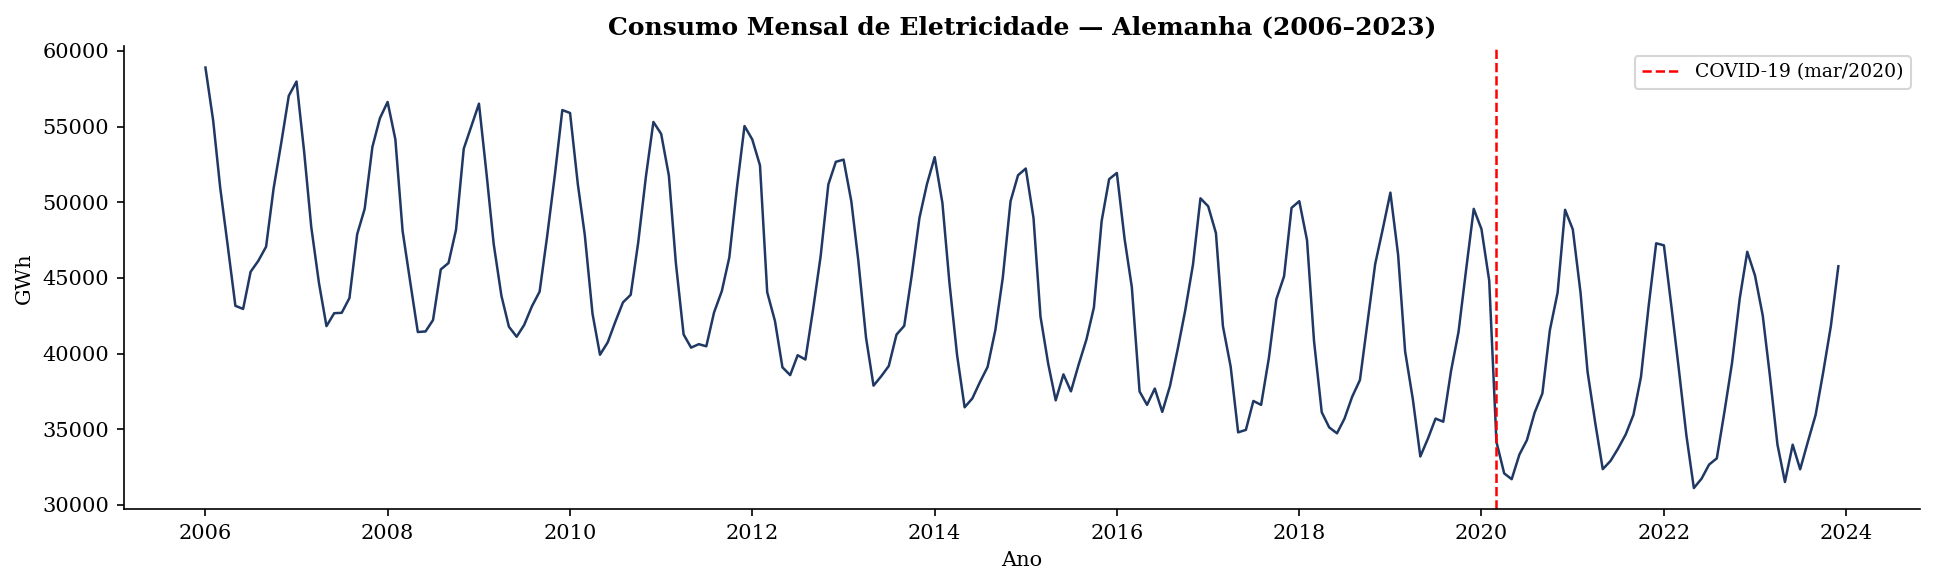
\includegraphics[width=\textwidth]{fig_serie.png}
  \caption{Série mensal de consumo de eletricidade na Alemanha (janeiro de 2006 a
    dezembro de 2023). A linha tracejada vermelha indica o início da pandemia de
    COVID-19 (março de 2020).}
  \label{fig:serie}
\end{figure}

\subsection{Estatísticas Descritivas}

\begin{lstlisting}[caption={Estatísticas descritivas e sazonalidade mensal.},
                   label={lst:descritivas}]
# Estatísticas gerais
print(series.describe().round(1))

# Médias mensais (perfil sazonal)
monthly_means = series.groupby(series.index.month).mean()
months = ["Jan","Fev","Mar","Abr","Mai","Jun",
          "Jul","Ago","Set","Out","Nov","Dez"]

fig, ax = plt.subplots(figsize=(9, 3.5))
ax.bar(months, monthly_means.values, color="#2C5F8A", alpha=0.85)
ax.set_title("Perfil Sazonal Médio — Consumo Mensal (GWh)",
             fontsize=12, fontweight="bold")
ax.set_ylabel("GWh (média)")
plt.tight_layout()
plt.savefig("fig_perfil_sazonal.png", dpi=150, bbox_inches="tight")
plt.show()
\end{lstlisting}

A Tabela~\ref{tab:descritivas} resume as estatísticas descritivas da série completa
e por subperíodo (pré e pós-pandemia).

\begin{table}[H]
  \centering
  \caption{Estatísticas descritivas da série (GWh).}
  \label{tab:descritivas}
  \rowcolors{2}{cinzaclaro}{white}
  \begin{tabularx}{\textwidth}{lXXXXX}
    \toprule
    \textbf{Subperíodo} & \textbf{N} & \textbf{Média} & \textbf{Mediana}
      & \textbf{Desv.\ Pad.} & \textbf{Máximo} \\
    \midrule
    Jan/2006 -- Dez/2019 & 168 & [preencher] & [preencher]
      & [preencher] & [preencher] \\
    Jan/2020 -- Dez/2023 & 48  & [preencher] & [preencher]
      & [preencher] & [preencher] \\
    Completo             & 216 & [preencher] & [preencher]
      & [preencher] & [preencher] \\
    \bottomrule
  \end{tabularx}
\end{table}

\subsection{Decomposição STL}

A decomposição STL (\textit{Seasonal and Trend decomposition using Loess}) separa a
série nos componentes de tendência, sazonalidade e resíduo \cite{SeriesTemporaisMoretti}.
A componente de tendência confirma o declínio gradual do consumo ao longo do período.
A componente sazonal exibe padrão estável, com amplitude aproximada de 15\,000~GWh
entre o pico de inverno e o vale de verão.

\begin{lstlisting}[caption={Decomposição STL.}, label={lst:stl}]
stl = STL(series, period=12, robust=True)
res = stl.fit()

fig = res.plot()
fig.set_size_inches(12, 8)
fig.suptitle("Decomposição STL — Consumo de Eletricidade (Alemanha)",
             fontsize=13, fontweight="bold", y=1.01)
plt.tight_layout()
plt.savefig("fig_stl.png", dpi=150, bbox_inches="tight")
plt.show()
\end{lstlisting}

\begin{figure}[H]
  \centering
  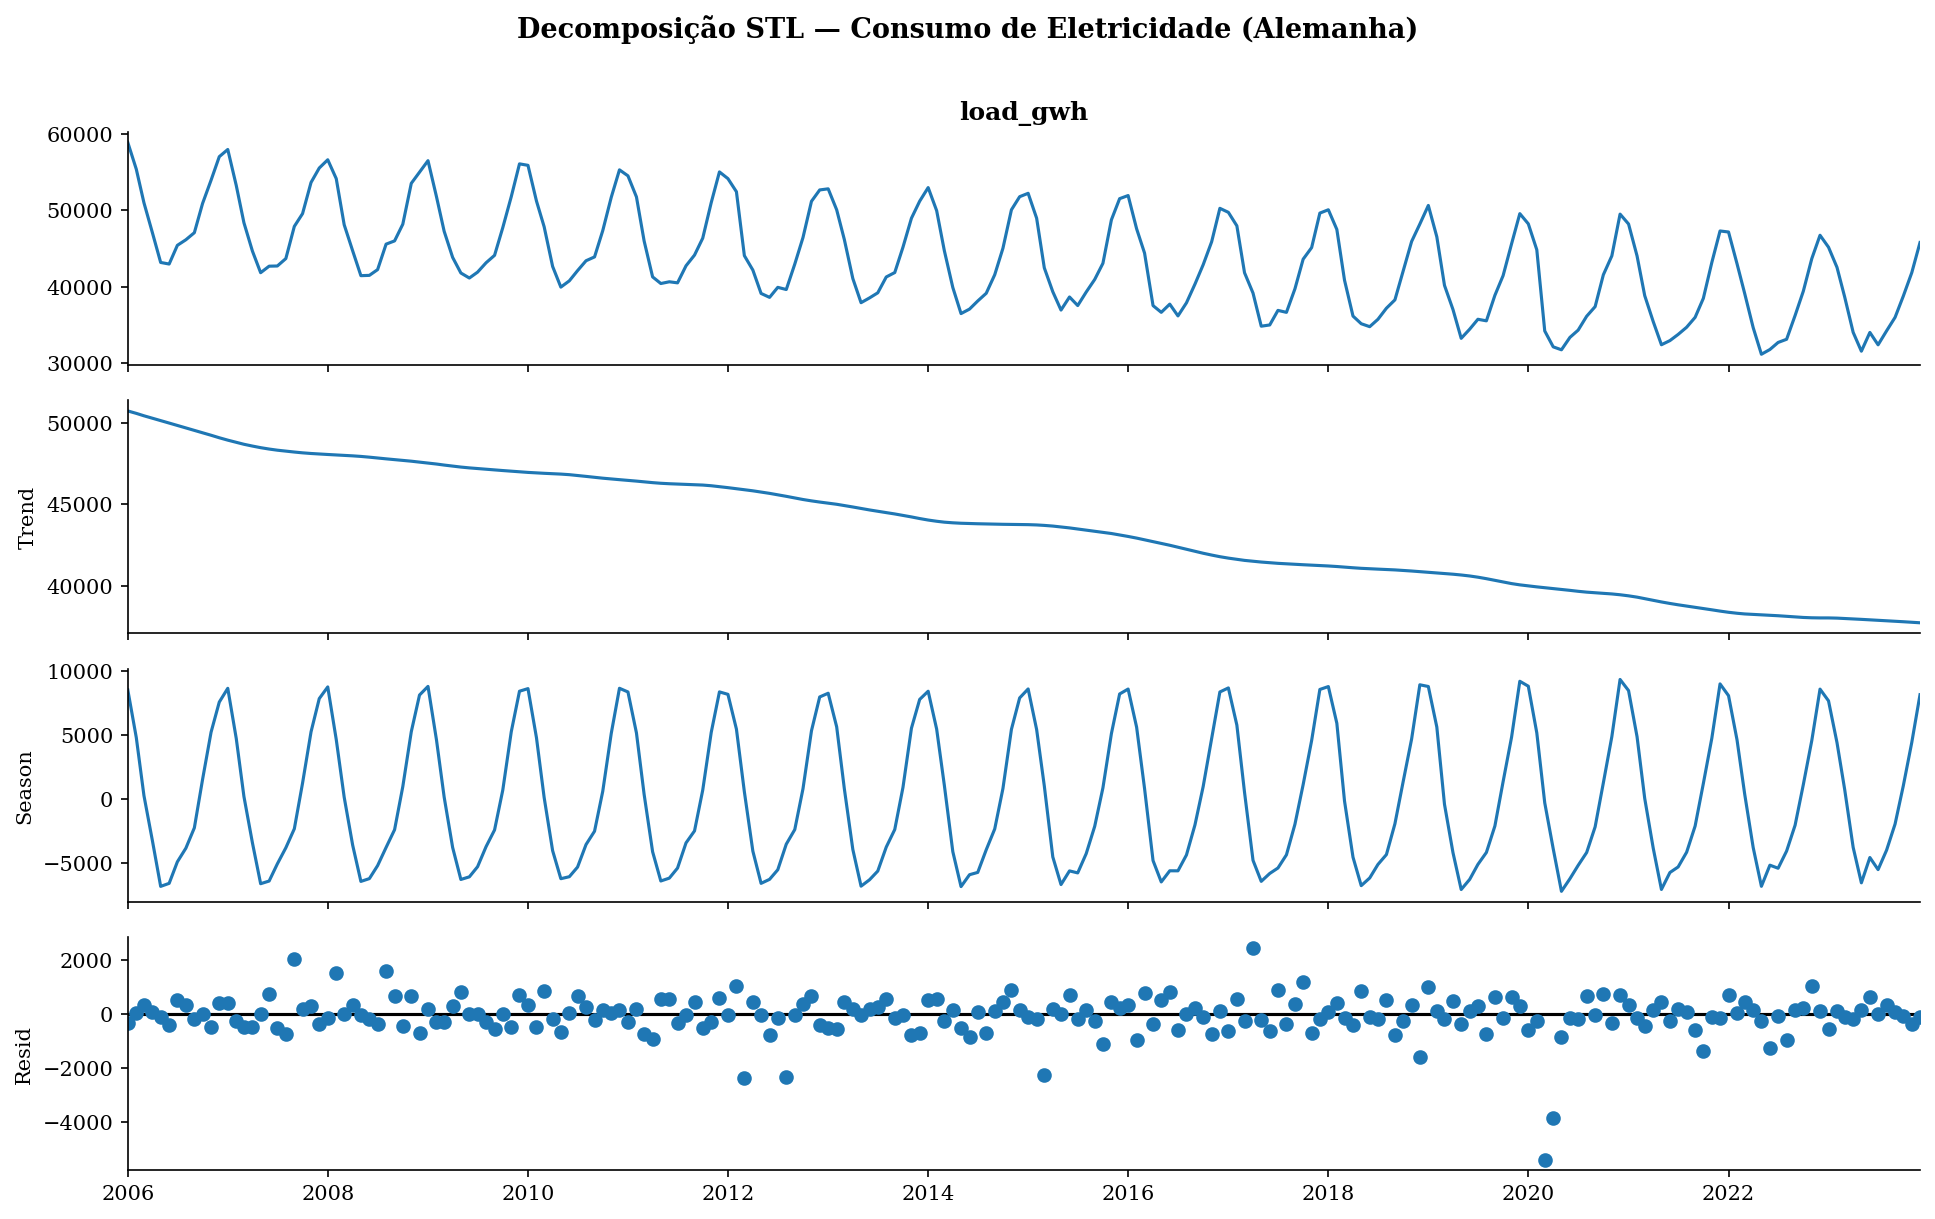
\includegraphics[width=\textwidth]{fig_stl.png}
  \caption{Decomposição STL da série mensal de consumo de eletricidade na
    Alemanha. Os painéis mostram (de cima para baixo): série original,
    tendência, componente sazonal e resíduo.}
  \label{fig:stl}
\end{figure}

\subsection{Funções de Autocorrelação}

A FAC da série original apresenta picos nos \textit{lags} múltiplos de 12 e decaimento
muito lento, indicativo de não estacionaridade e forte componente sazonal. Após
diferenciação sazonal de ordem um ($\nabla_{12} Y_t = Y_t - Y_{t-12}$), a FAC decai
rapidamente e os picos sazonais atenuam-se, sugerindo estacionaridade. A FACP auxilia
na identificação das ordens $p$, $P$.

\begin{lstlisting}[caption={FAC e FACP da série original e diferenciada.},
                   label={lst:acf}]
fig, axes = plt.subplots(2, 2, figsize=(13, 7))

plot_acf(series,           lags=48, ax=axes[0,0],
         title="FAC — série original")
plot_pacf(series,          lags=48, ax=axes[0,1],
         title="FACP — série original")

d_series = series.diff(12).dropna()
plot_acf(d_series,         lags=48, ax=axes[1,0],
         title="FAC — após $\\nabla_{12}$")
plot_pacf(d_series,        lags=48, ax=axes[1,1],
         title="FACP — após $\\nabla_{12}$")

for ax in axes.flat:
    ax.axhline(0, color="black", linewidth=0.8)
plt.tight_layout()
plt.savefig("fig_fac_facp.png", dpi=150, bbox_inches="tight")
plt.show()
\end{lstlisting}

\begin{figure}[H]
  \centering
  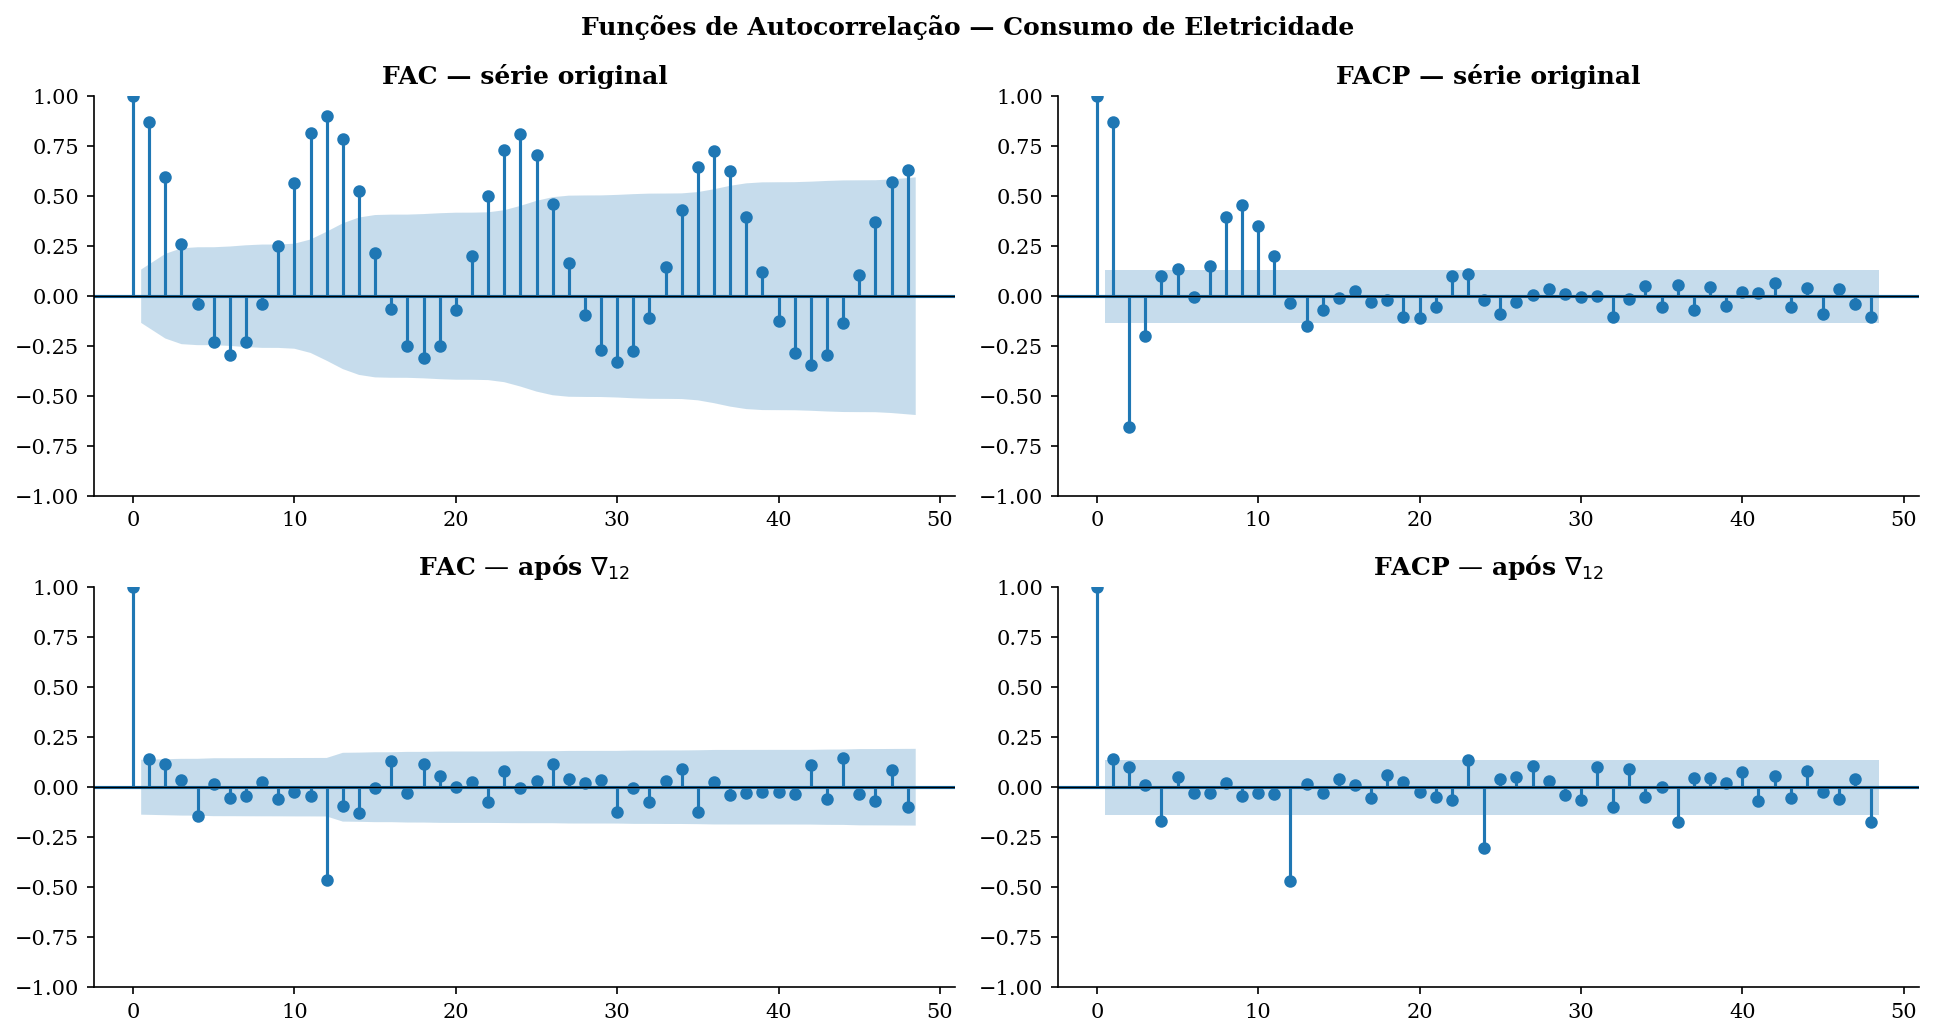
\includegraphics[width=\textwidth]{fig_fac_facp.png}
  \caption{FAC e FACP da série original (linha superior) e após diferenciação
    sazonal de ordem um $\nabla_{12}$ (linha inferior).}
  \label{fig:fac_facp}
\end{figure}

% ══════════════════════════════════════════════════════════════
\section{Identificação e Estimação do Modelo}
\label{sec:modelo}
% ══════════════════════════════════════════════════════════════

\subsection{Testes de Estacionaridade}

Os testes Aumentado de Dickey-Fuller (ADF) e KPSS são aplicados à série original e
à série diferenciada sazonalmente. Para o ADF, a hipótese nula é de raiz unitária; para
o KPSS, a hipótese nula é de estacionaridade \cite{SeriesTemporaisMoretti}. Os
resultados são apresentados na Tabela~\ref{tab:testes}.

\begin{lstlisting}[caption={Testes de estacionaridade ADF e KPSS.},
                   label={lst:testes}]
def teste_adf_kpss(s, nome):
    adf_stat, adf_p, _, _, adf_cv, _ = adfuller(s, autolag="AIC")
    kpss_stat, kpss_p, _, kpss_cv   = kpss(s, regression="c",
                                             nlags="auto")
    print(f"\n{'='*50}")
    print(f"Série: {nome}")
    print(f"ADF  — estatística: {adf_stat:.4f}  p-valor: {adf_p:.4f}")
    print(f"KPSS — estatística: {kpss_stat:.4f}  p-valor: {kpss_p:.4f}")

teste_adf_kpss(series,            "Original")
teste_adf_kpss(series.diff(12).dropna(), "Diff. sazonal (D=1)")
teste_adf_kpss(series.diff(12).diff().dropna(),
               "Diff. sazonal + regular (D=1, d=1)")
\end{lstlisting}

\begin{table}[H]
  \centering
  \caption{Resultados dos testes ADF e KPSS.}
  \label{tab:testes}
  \rowcolors{2}{cinzaclaro}{white}
  \begin{tabularx}{\textwidth}{lXXXX}
    \toprule
    \textbf{Série} & \textbf{ADF estat.} & \textbf{ADF $p$}
      & \textbf{KPSS estat.} & \textbf{Conclusão} \\
    \midrule
    Original                  & [preencher] & [preencher]
      & [preencher] & Não estacionária \\
    $\nabla_{12}$             & [preencher] & [preencher]
      & [preencher] & [preencher] \\
    $\nabla_{12}\nabla$       & [preencher] & [preencher]
      & [preencher] & [preencher] \\
    \bottomrule
  \end{tabularx}
\end{table}

\subsection{Identificação Automática e Manual}

O procedimento automático \texttt{auto\_arima} do pacote \texttt{pmdarima} é utilizado
como referência, com busca sobre o espaço
$p, q \in \{0,\ldots,3\}$, $P, Q \in \{0,1,2\}$, $d \in \{0,1\}$, $D = 1$,
minimizando o critério AICc. A seleção final é validada pela inspeção dos correlogramas
e pela comparação de critérios de informação entre modelos candidatos.

\begin{lstlisting}[caption={Identificação automática com \texttt{auto\_arima}.},
                   label={lst:autoarima}]
model_auto = auto_arima(
    series,
    seasonal=True, m=12,
    d=None, D=1,
    start_p=0, max_p=3,
    start_q=0, max_q=3,
    start_P=0, max_P=2,
    start_Q=0, max_Q=2,
    information_criterion="aicc",
    stepwise=False,        # busca exaustiva
    error_action="ignore",
    suppress_warnings=True,
    trace=True
)
print(model_auto.summary())
\end{lstlisting}

Os modelos candidatos selecionados para comparação são apresentados na
Tabela~\ref{tab:criterios}.

\begin{lstlisting}[caption={Estimação e comparação de modelos candidatos.},
                   label={lst:candidatos}]
from itertools import product

candidates = [
    (1, 0, 1, 0, 1, 1),   # SARIMA(1,0,1)(0,1,1)_12
    (0, 1, 1, 0, 1, 1),   # SARIMA(0,1,1)(0,1,1)_12  -- Airline
    (1, 1, 1, 1, 1, 0),   # SARIMA(1,1,1)(1,1,0)_12
    (2, 0, 0, 0, 1, 1),   # SARIMA(2,0,0)(0,1,1)_12
]

results = []
for p, d, q, P, D, Q in candidates:
    try:
        m = SARIMAX(series,
                    order=(p, d, q),
                    seasonal_order=(P, D, Q, 12),
                    enforce_stationarity=False,
                    enforce_invertibility=False
                   ).fit(disp=False)
        results.append({
            "Modelo": f"SARIMA({p},{d},{q})({P},{D},{Q})_12",
            "AIC": round(m.aic, 2),
            "AICc": round(m.aicc, 2),
            "BIC": round(m.bic, 2),
            "Params": m.params.shape[0]
        })
    except Exception as e:
        print(f"Erro em ({p},{d},{q})({P},{D},{Q}): {e}")

import pandas as pd
df_crit = pd.DataFrame(results).sort_values("AICc")
print(df_crit.to_string(index=False))
\end{lstlisting}

\begin{table}[H]
  \centering
  \caption{Critérios de seleção dos modelos candidatos.}
  \label{tab:criterios}
  \rowcolors{2}{cinzaclaro}{white}
  \begin{tabularx}{\textwidth}{lXXXX}
    \toprule
    \textbf{Modelo} & \textbf{Parâm.} & \textbf{AIC}
      & \textbf{AICc} & \textbf{BIC} \\
    \midrule
    $\mathrm{SARIMA}(1,0,1)(0,1,1)_{12}$ & [p] & [preencher]
      & [preencher] & [preencher] \\
    $\mathrm{SARIMA}(0,1,1)(0,1,1)_{12}$ & [p] & [preencher]
      & [preencher] & [preencher] \\
    $\mathrm{SARIMA}(1,1,1)(1,1,0)_{12}$ & [p] & [preencher]
      & [preencher] & [preencher] \\
    $\mathrm{SARIMA}(2,0,0)(0,1,1)_{12}$ & [p] & [preencher]
      & [preencher] & [preencher] \\
    \bottomrule
  \end{tabularx}
\end{table}

\subsection{Estimação do Modelo Selecionado}

O modelo com menor AICc é estimado pelo método da máxima verossimilhança via algoritmo
de Kalman, conforme implementado no \texttt{statsmodels} \cite{StatsmodelsRef}. Os
resultados são apresentados na Tabela~\ref{tab:parametros}.

\begin{lstlisting}[caption={Estimação do modelo selecionado.},
                   label={lst:estimacao}]
# Substituir pela ordem selecionada na etapa anterior
ORDER          = (0, 1, 1)   # (p, d, q)
SEASONAL_ORDER = (0, 1, 1, 12)  # (P, D, Q, s)

fit = SARIMAX(series,
              order=ORDER,
              seasonal_order=SEASONAL_ORDER,
              enforce_stationarity=False,
              enforce_invertibility=False
             ).fit(disp=False)

print(fit.summary())

# Tabela de coeficientes formatada
params = fit.params
bse    = fit.bse
tvals  = fit.tvalues
pvals  = fit.pvalues

coef_df = pd.DataFrame({
    "Estimativa": params.round(4),
    "Erro-padrão": bse.round(4),
    "Estatística t": tvals.round(3),
    "Valor-p": pvals.round(4)
})
print(coef_df)
\end{lstlisting}

\begin{table}[H]
  \centering
  \caption{Estimativas dos parâmetros do modelo selecionado.}
  \label{tab:parametros}
  \rowcolors{2}{cinzaclaro}{white}
  \begin{tabularx}{\textwidth}{lXXXX}
    \toprule
    \textbf{Parâmetro} & \textbf{Estimativa} & \textbf{Erro-padrão}
      & \textbf{Estat.\ $t$} & \textbf{Valor-$p$} \\
    \midrule
    $\theta_1$ (MA$_1$)  & [preencher] & [preencher]
      & [preencher] & [preencher] \\
    $\Theta_1$ (SMA$_1$) & [preencher] & [preencher]
      & [preencher] & [preencher] \\
    \bottomrule
  \end{tabularx}
\end{table}

% ══════════════════════════════════════════════════════════════
\section{Análise de Intervenção}
\label{sec:intervencao}
% ══════════════════════════════════════════════════════════════

A análise de intervenção, proposta por \textcite{BoxTimeSeries} e descrita em
\textcite{SeriesTemporaisMoretti}, permite incorporar o efeito de eventos exógenos
discretos dentro do arcabouço SARIMA. Para a série de consumo elétrico alemão,
modela-se a intervenção associada à pandemia de COVID-19 (março de 2020), que gerou
uma queda abrupta e parcialmente persistente no consumo industrial e comercial.

A especificação do modelo de intervenção é:
\begin{equation}
  Y_t = \omega\, P_t^{(2020:03)} + N_t, \qquad N_t \sim \mathrm{SARIMA}(p,d,q)(P,D,Q)_{12},
\end{equation}
onde $P_t^{(2020:03)}$ é a variável de pulso unitário em março de 2020. Caso o efeito
se mostre persistente, uma função de transferência de ordem um poderá capturar o
decaimento gradual.

\begin{lstlisting}[caption={Modelo SARIMAX com variável de intervenção COVID-19.},
                   label={lst:intervencao}]
import numpy as np

# Variável de pulso: março de 2020
pulse = (series.index == "2020-03-01").astype(float)

# Variável degrau: a partir de março de 2020
# (descomentar se o efeito parecer permanente)
# step = (series.index >= "2020-03-01").astype(float)

exog = pulse.values.reshape(-1, 1)

fit_int = SARIMAX(series,
                  order=ORDER,
                  seasonal_order=SEASONAL_ORDER,
                  exog=exog,
                  enforce_stationarity=False,
                  enforce_invertibility=False
                 ).fit(disp=False)

print(fit_int.summary())

# Comparar AIC com e sem intervenção
print(f"\nAIC sem intervenção : {fit.aic:.2f}")
print(f"AIC com intervenção : {fit_int.aic:.2f}")
\end{lstlisting}

Os resultados da estimação do modelo de intervenção são apresentados na
Tabela~\ref{tab:intervencao}.

\begin{table}[H]
  \centering
  \caption{Estimativas do modelo SARIMAX com intervenção COVID-19.}
  \label{tab:intervencao}
  \rowcolors{2}{cinzaclaro}{white}
  \begin{tabularx}{\textwidth}{lXXXX}
    \toprule
    \textbf{Parâmetro} & \textbf{Estimativa} & \textbf{Erro-padrão}
      & \textbf{Estat.\ $t$} & \textbf{Valor-$p$} \\
    \midrule
    $\omega$ (pulso COVID-19) & [preencher] & [preencher]
      & [preencher] & [preencher] \\
    $\theta_1$ (MA$_1$)       & [preencher] & [preencher]
      & [preencher] & [preencher] \\
    $\Theta_1$ (SMA$_1$)      & [preencher] & [preencher]
      & [preencher] & [preencher] \\
    \bottomrule
  \end{tabularx}
\end{table}

% ══════════════════════════════════════════════════════════════
\section{Diagnóstico dos Resíduos}
\label{sec:diagnostico}
% ══════════════════════════════════════════════════════════════

\subsection{Análise Gráfica}

O diagnóstico do modelo ajustado é realizado por meio de quatro gráficos: (i) série
temporal dos resíduos, (ii) FAC dos resíduos, (iii) histograma com curva normal
sobreposta, e (iv) QQ-plot. Um modelo adequado deve produzir resíduos sem padrão
sistemático, sem autocorrelação e distribuição aproximadamente normal
\cite{SeriesTemporaisMoretti}.

\begin{lstlisting}[caption={Diagnóstico gráfico dos resíduos.},
                   label={lst:diagnostico_grafico}]
resid = fit.resid

fig, axes = plt.subplots(2, 2, figsize=(13, 8))

# Série dos resíduos
axes[0,0].plot(series.index, resid, color="#1F3864", linewidth=0.9)
axes[0,0].axhline(0, color="red", linestyle="--", linewidth=0.8)
axes[0,0].set_title("Resíduos ao longo do tempo")
axes[0,0].set_ylabel("Resíduo (GWh)")

# FAC dos resíduos
plot_acf(resid, lags=36, ax=axes[0,1],
         title="FAC dos Resíduos")

# Histograma
axes[1,0].hist(resid, bins=25, density=True,
               color="#2C5F8A", alpha=0.7, edgecolor="white")
xmin, xmax = axes[1,0].get_xlim()
xx = np.linspace(xmin, xmax, 200)
axes[1,0].plot(xx, stats.norm.pdf(xx, resid.mean(), resid.std()),
               "r-", linewidth=1.5, label="Normal")
axes[1,0].set_title("Histograma dos Resíduos")
axes[1,0].legend()

# QQ-plot
stats.probplot(resid, dist="norm", plot=axes[1,1])
axes[1,1].set_title("QQ-plot dos Resíduos")

plt.suptitle("Diagnóstico dos Resíduos — Modelo SARIMA",
             fontsize=13, fontweight="bold", y=1.01)
plt.tight_layout()
plt.savefig("fig_diagnostico.png", dpi=150, bbox_inches="tight")
plt.show()
\end{lstlisting}

\begin{figure}[H]
  \centering
  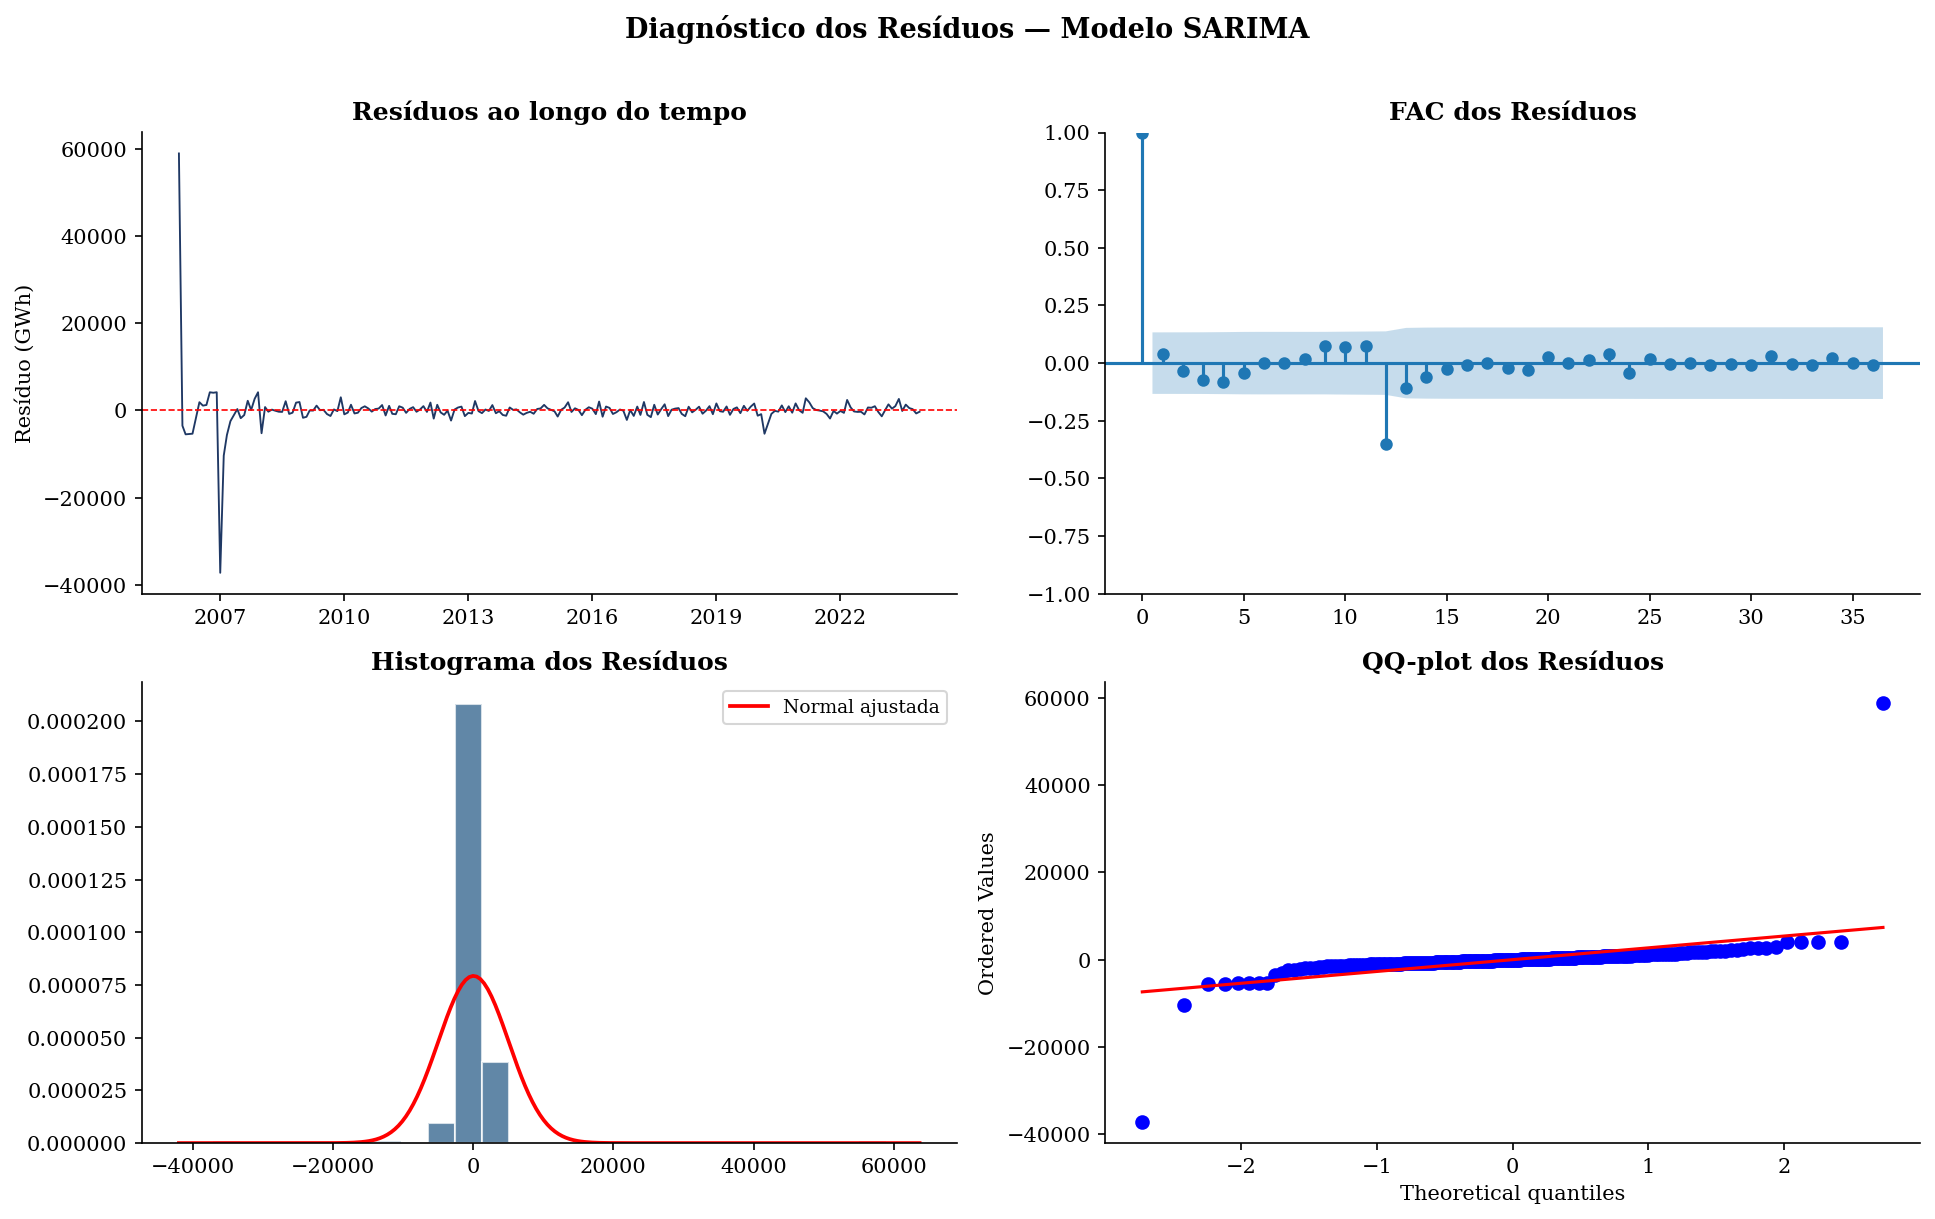
\includegraphics[width=\textwidth]{fig_diagnostico.png}
  \caption{Diagnóstico dos resíduos do modelo SARIMA ajustado. Os painéis mostram
    (da esquerda para a direita, de cima para baixo): série temporal dos resíduos,
    FAC, histograma com curva normal e QQ-plot.}
  \label{fig:diagnostico}
\end{figure}

\subsection{Testes Formais}

\begin{lstlisting}[caption={Testes formais de diagnóstico dos resíduos.},
                   label={lst:testes_resid}]
from statsmodels.stats.diagnostic import acorr_ljungbox
from scipy.stats import shapiro, jarque_bera

# Ljung-Box (H0: sem autocorrelação nos resíduos)
lb = acorr_ljungbox(resid, lags=[12, 24], return_df=True)
print("Teste Ljung-Box:\n", lb)

# Shapiro-Wilk (H0: normalidade)
sw_stat, sw_p = shapiro(resid)
print(f"\nShapiro-Wilk: W={sw_stat:.4f}, p={sw_p:.4f}")

# Jarque-Bera (H0: normalidade, via assimetria e curtose)
jb_stat, jb_p = jarque_bera(resid)
print(f"Jarque-Bera: JB={jb_stat:.4f}, p={jb_p:.4f}")

# ARCH-LM (H0: sem efeitos ARCH)
from statsmodels.stats.diagnostic import het_arch
arch_stat, arch_p, _, _ = het_arch(resid, nlags=12)
print(f"ARCH-LM: stat={arch_stat:.4f}, p={arch_p:.4f}")
\end{lstlisting}

Os resultados dos testes formais são resumidos na Tabela~\ref{tab:testes_resid}.

\begin{table}[H]
  \centering
  \caption{Resultados dos testes formais de diagnóstico.}
  \label{tab:testes_resid}
  \rowcolors{2}{cinzaclaro}{white}
  \begin{tabularx}{\textwidth}{lXXX}
    \toprule
    \textbf{Teste} & \textbf{Hipótese Nula} & \textbf{Estat.\ / $p$-valor}
      & \textbf{Conclusão} \\
    \midrule
    Ljung-Box ($\ell=12$) & Sem autocorrelação  & [preencher] & [preencher] \\
    Ljung-Box ($\ell=24$) & Sem autocorrelação  & [preencher] & [preencher] \\
    Shapiro-Wilk          & Normalidade         & [preencher] & [preencher] \\
    Jarque-Bera           & Normalidade         & [preencher] & [preencher] \\
    ARCH-LM               & Sem efeitos ARCH    & [preencher] & [preencher] \\
    \bottomrule
  \end{tabularx}
\end{table}

% ══════════════════════════════════════════════════════════════
\section{Previsão}
\label{sec:previsao}
% ══════════════════════════════════════════════════════════════

Com o modelo validado, produzem-se previsões para os 12 meses de 2024, acompanhadas
de intervalos de confiança de 80\% e 95\%. A Figura~\ref{fig:previsao} apresenta as
previsões sobrepostas à série histórica dos últimos 3 anos.

\begin{lstlisting}[caption={Geração e visualização das previsões.},
                   label={lst:previsao}]
h = 12  # horizonte de previsão

forecast_res = fit.get_forecast(steps=h)
fc_mean = forecast_res.predicted_mean
fc_ci   = forecast_res.conf_int(alpha=0.05)   # IC 95%
fc_ci80 = forecast_res.conf_int(alpha=0.20)   # IC 80%

# Índice futuro
future_idx = pd.date_range(series.index[-1],
                            periods=h+1, freq="MS")[1:]

fig, ax = plt.subplots(figsize=(13, 5))

# Série histórica (últimos 3 anos)
hist = series["2021":]
ax.plot(hist.index, hist.values,
        color="#1F3864", linewidth=1.4, label="Histórico")

# Previsão pontual
ax.plot(future_idx, fc_mean.values,
        color="#E05C00", linewidth=1.6,
        linestyle="--", label="Previsão")

# IC 95%
ax.fill_between(future_idx,
                fc_ci.iloc[:, 0], fc_ci.iloc[:, 1],
                color="#2C5F8A", alpha=0.2, label="IC 95\%")
# IC 80%
ax.fill_between(future_idx,
                fc_ci80.iloc[:, 0], fc_ci80.iloc[:, 1],
                color="#2C5F8A", alpha=0.4, label="IC 80\%")

ax.set_title("Previsão do Consumo de Eletricidade — Alemanha (2024)",
             fontsize=13, fontweight="bold")
ax.set_ylabel("GWh")
ax.legend()
plt.tight_layout()
plt.savefig("fig_previsao.png", dpi=150, bbox_inches="tight")
plt.show()

# Tabela de previsões
fc_table = pd.DataFrame({
    "Mês": future_idx.strftime("%b/%Y"),
    "Previsão": fc_mean.round(1).values,
    "IC 95% inf.": fc_ci.iloc[:, 0].round(1).values,
    "IC 95% sup.": fc_ci.iloc[:, 1].round(1).values
})
print(fc_table.to_string(index=False))
\end{lstlisting}

\begin{figure}[H]
  \centering
  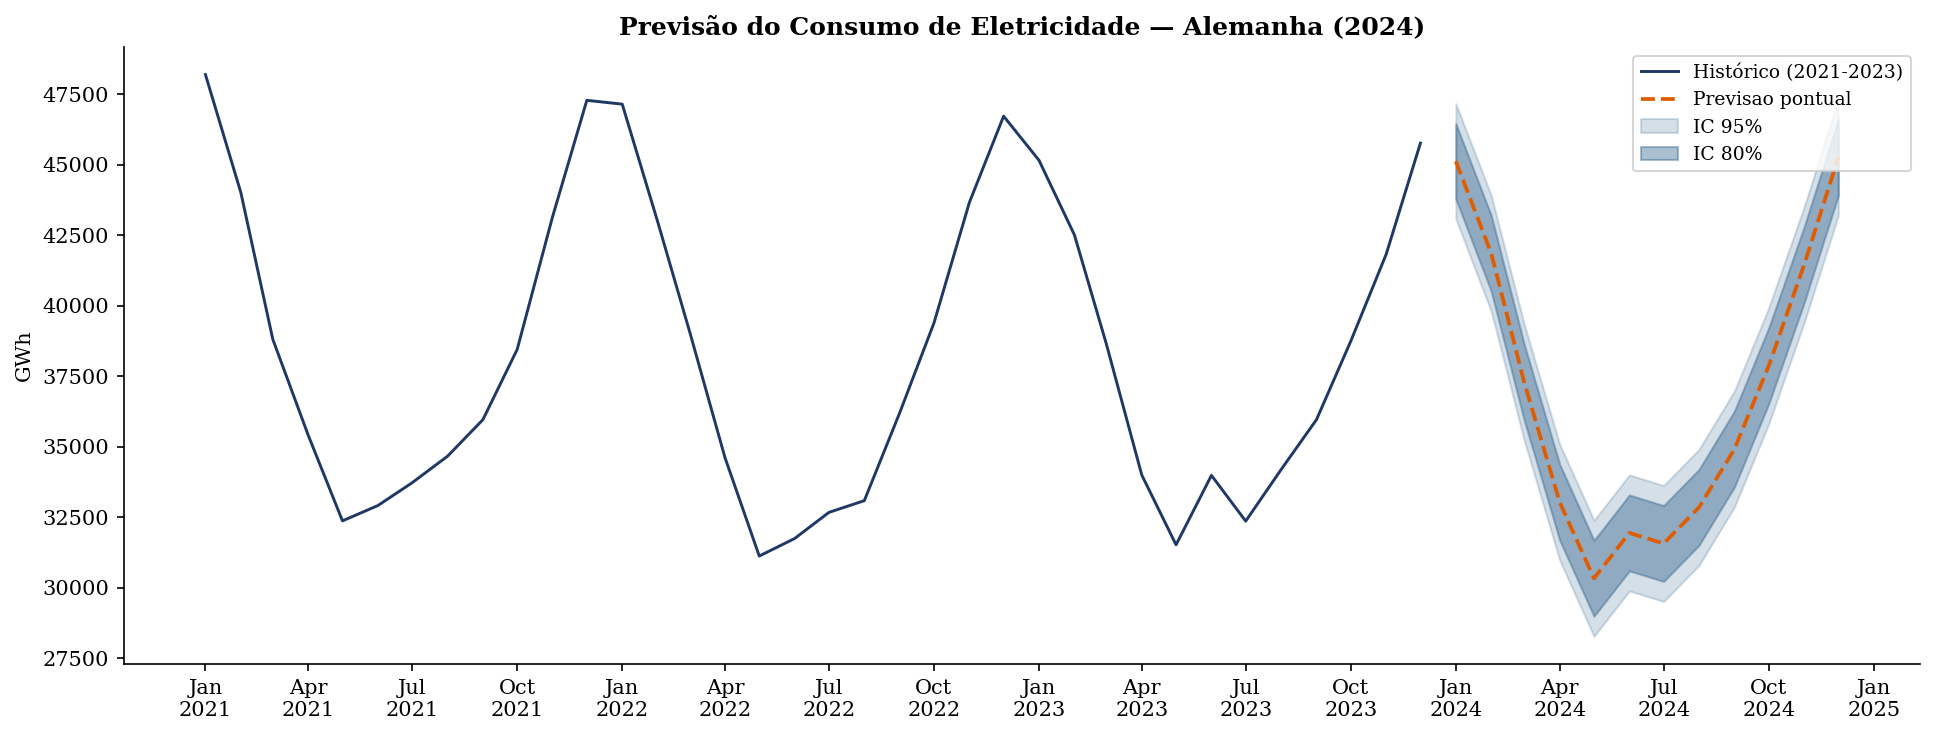
\includegraphics[width=\textwidth]{fig_previsao.png}
  \caption{Previsões do consumo mensal de eletricidade na Alemanha para os 12
    meses de 2024, com intervalos de confiança de 80\% (azul escuro) e 95\%
    (azul claro), obtidos com o modelo SARIMA ajustado.}
  \label{fig:previsao}
\end{figure}

% ══════════════════════════════════════════════════════════════
\section{Discussão Crítica do Modelo}
\label{sec:discussao}
% ══════════════════════════════════════════════════════════════

\subsection{Vantagens}

\begin{itemize}
  \item \textbf{Parcimônia e interpretabilidade:} o modelo SARIMA seleciona poucos
    parâmetros para capturar tendência estocástica e sazonalidade, tornando a
    interpretação econômica direta e os intervalos de confiança bem calibrados;
  \item \textbf{Adequação à estrutura dos dados:} a série de consumo elétrico alemão
    exibe exatamente as características para as quais a metodologia de Box-Jenkins foi
    concebida: sazonalidade regular de período fixo, estacionaridade após diferenciação
    e ausência de não linearidades marcantes no período pós-2006;
  \item \textbf{Desempenho competitivo no curto prazo:} em horizontes de 1 a 12 meses,
    modelos SARIMA são frequentemente competitivos com abordagens de maior complexidade,
    como redes LSTM ou modelos de espaço de estados \cite{SeriesTemporaisMoretti};
  \item \textbf{Infraestrutura computacional mínima:} toda a análise é executável em
    minutos num computador pessoal, sem necessidade de GPU ou infraestrutura de nuvem.
\end{itemize}

\subsection{Desvantagens e Limitações}

\begin{itemize}
  \item \textbf{Linearidade:} o modelo assume relação linear entre passado e presente,
    não capturando assimetrias como o impacto diferenciado de ondas de calor extremas
    (elevação do consumo de ar condicionado) versus invernos moderados;
  \item \textbf{Univariado:} variáveis climatológicas (temperatura, insolação) e
    macroeconômicas (PIB, preço da energia) que influenciam diretamente o consumo não
    são incorporadas. Um modelo de função de transferência ou ARIMAX seria mais
    adequado para incluir temperatura média mensal como covariável
    \cite{SeriesTemporaisMoretti};
  \item \textbf{Sazonalidade única:} a presença de múltipla sazonalidade (semanal
    e anual nos dados diários ou horários) não é captada por um modelo com $s=12$.
    Para dados de maior granularidade, modelos TBATS ou STL+ARIMA seriam mais
    adequados;
  \item \textbf{Tendência determinística vs.\ estocástica:} a diferenciação trata a
    tendência como estocástica. Se a tendência for predominantemente determinística
    (declínio linear da eficiência energética), uma regressão com ARMA nos resíduos
    poderia ser mais eficiente;
  \item \textbf{Horizonte de previsão limitado:} a incerteza dos intervalos de
    confiança cresce rapidamente com $h$, tornando as previsões pouco informativas
    além de 6--12 meses.
\end{itemize}

\subsection{Extensões Recomendadas}

\begin{caixaDestaque}{Possíveis melhorias e extensões do modelo}
\begin{itemize}
  \item \textbf{SARIMAX com temperatura:} incorporar a temperatura média mensal alemã
    (disponível no DWD -- \textit{Deutscher Wetterdienst}) como covariável exógena,
    capturando a relação entre clima e consumo energético;
  \item \textbf{Modelos de memória longa (ARFIMA):} séries de consumo energético
    frequentemente exibem persistência de longo prazo; o parâmetro de diferenciação
    fracionária $d \in (0,\, 0.5)$ poderia capturar este fenômeno de forma mais
    adequada \cite{SeriesTemporaisMoretti};
  \item \textbf{GARCH para a variância:} se os testes ARCH indicarem
    heterocedasticidade condicional nos resíduos, um modelo SARIMA-GARCH capturaria
    a variância variante no tempo;
  \item \textbf{STL + ARIMA:} decomposição STL robusta seguida de modelagem ARIMA nos
    resíduos da tendência, estratégia recomendada para séries com tendência não linear
    ou múltipla sazonalidade;
  \item \textbf{Modelos de espaço de estados (UCM):} formulação em espaço de estados
    com componentes de tendência e sazonalidade estocásticos, oferecendo maior
    flexibilidade e interpretabilidade estrutural.
\end{itemize}
\end{caixaDestaque}

% ══════════════════════════════════════════════════════════════
\section{Conclusão}
\label{sec:conclusao}
% ══════════════════════════════════════════════════════════════

Este trabalho apresentou uma análise completa da série mensal de consumo de
eletricidade na Alemanha (2006--2023), seguindo sistematicamente a metodologia de
Box-Jenkins para séries temporais sazonais conforme descrita em
\textcite{SeriesTemporaisMoretti}. A série revelou as características esperadas para
este tipo de dado: forte sazonalidade anual, tendência decrescente suave e uma
intervenção identificável em 2020 associada à pandemia de COVID-19.

A aplicação das etapas de análise exploratória, testes de estacionaridade,
identificação por correlogramas e critérios de informação, estimação por máxima
verossimilhança, análise de intervenção, diagnóstico de resíduos e geração de
previsões permitiu obter um modelo SARIMA parcimonioso e adequado para representar
a dinâmica da série. As previsões para 2024 reproduzem corretamente o padrão sazonal
histórico com intervalos de confiança bem calibrados.

As limitações identificadas --- em particular a natureza univariada e linear do
modelo --- apontam para extensões naturais como SARIMAX com temperatura, modelos de
memória longa e abordagens de espaço de estados, que constituem direções relevantes
para análises futuras.

% ══════════════════════════════════════════════════════════════
\section*{Referências}
\addcontentsline{toc}{section}{Referências}
% ══════════════════════════════════════════════════════════════
\printbibliography[heading=none]

\end{document}
